\documentclass[10pt]{article}

\usepackage[T1]{fontenc}
\usepackage{geometry}
\usepackage{amsmath, amssymb, amsthm}
\usepackage[scr]{rsfso}
\usepackage{graphicx}

\usepackage{tikz}
\usetikzlibrary{positioning}
\tikzset{main node/.style={circle,fill=blue!20,draw,minimum size=1cm,inner sep=0pt}}
\tikzset{red node/.style={circle,fill=red!20,draw,minimum size=1cm,inner sep=0pt}}
\tikzset{green node/.style={circle,fill=green!20,draw,minimum size=1cm,inner sep=0pt}}

\geometry{a4paper, margin=1in}

\renewcommand{\labelenumi}{(\alph{enumi})}

\newcounter{prob}
\newcommand{\problem}{\stepcounter{prob}\paragraph{Exercise \arabic{prob}}}
\newcommand{\solution}{\paragraph{Solution}}

\newcommand{\C}{\mathbb{C}}
\newcommand{\R}{\mathbb{R}}
\newcommand{\Q}{\mathbb{Q}}
\newcommand{\Z}{\mathbb{Z}}
\newcommand{\N}{\mathbb{N}}

\DeclareMathOperator{\diam}{diam}
\DeclareMathOperator{\girth}{girth}
\DeclareMathOperator{\aut}{aut}

\newtheorem{theorem}{Theorem}
\newtheorem{lemma}{Lemma}

\title{MA3103: Introduction to Graph Theory and Combinatorics}
\author{Satvik Saha}
\date{}

\begin{document}
    \noindent\textbf{IISER Kolkata} \hfill \textbf{Assignment IV}
    \vspace{3pt}
    \hrule
    \vspace{3pt}
    \begin{center}
    \LARGE{\textbf{MA3101 : Introduction to Graph Theory and Combinatorics}}
    \end{center}
    \vspace{3pt}
    \hrule
    \vspace{3pt}
    Satvik Saha, \texttt{19MS154} \hfill \today
    \vspace{20pt}

    \problem Prove that the automorphism group of a graph $G$ is equal to the
    automorphism group if its complement $\overline{G}$.

    \solution Let $g \in \aut(G)$ be an automorphism, i.e.\ a permutation of the
    vertices of $G$; we claim that $g \in \aut(\overline{G})$. To see this, pick $x,
    y \in V$ (here, $V$ is the set of vertices, common to $G$ and $\overline{G}$).
    There are two possible cases: \\
    
    \textbf{Case I}: $x \sim y$ in $\overline{G}$. This means that $x \not\sim y$ in
    $G$, hence $g(x) \not\sim g(y)$ in $G$. Thus, $g(x) \sim g(y)$ in $\overline{G}$.

    \textbf{Case II}: $x \not\sim y$ in $\overline{G}$. This means that $x \sim y$ in
    $G$, hence $g(x) \sim g(y)$ in $G$. Thus, $g(x) \not\sim g(y)$ in $\overline{G}$.
    \\

    In either case, $g$ preserves the adjacency relationships between vertices in
    $\overline{G}$. This shows that $\aut(\overline{G}) \subseteq \aut(G)$. Exactly
    the same argument can be repeated, interchanging the roles of $G$ and
    $\overline{G}$; or simply note that $\overline{\overline{G}} = G$ to conclude
    that $\aut(\overline{\overline{G}}) \subseteq \aut(\overline{G}) \subseteq
    \aut{G}$ gives $\aut(G) = \aut(\overline{G})$.


    \problem If $x$ and $y$ are vertices of $X$ and $g \in \aut(X)$, prove that $d(x,
    y) = d(g(x), g(y))$.

    \solution First suppose that $x$ and $y$ are not connected, i.e.\ there is no
    path joining them. If $g(x)$ and $g(y)$ were connected, that would give a path
    $g(x) \sim v_1 \sim \dots \sim v_k \sim g(y)$; now, applying the automorphism
    $g^{-1}$ gives a path $x \sim g^{-1}(v_1) \sim \dots \sim g^{-1}(v_k) \sim y$, a
    contradiction. Thus, $d(x, y) = \infty$ implies that $d(g(x), g(y)) = \infty$.
    Conversely, if $g(x)$ and $g(y)$ are not connected but $x$ and $y$ are via some
    path, applying $g$ to that path yields a path between $g(x)$ and $g(y)$ exactly
    as before. Thus, $d(g(x), g(y)) = \infty$ also implies that $d(x, y) = \infty$.

    Let $d(x, y) = k + 1 < \infty$ (we have $k \geq 0$). This means that there exists
    a path $x \sim v_1 \sim \dots \sim v_k \sim y$. Applying $g$ yields a path $g(x)
    \sim g(v_1) \sim \dots \sim g(v_k) \sim g(y)$, hence $d(g(x), g(y)) \leq d(x,
    y)$. Now if there was a shorter path $g(x) \sim u_1 \sim \dots \sim u_l \sim
    g(y)$, $l < k$ applying $g^{-1}$ would give the shorter path $x \sim g^{-1}(u_1)
    \sim \dots \sim g^{-1}(u_l) \sim y$ between $x$ and $y$, contradicting the
    minimality of $d(x, y) = k + 1$. Thus, $d(x, y) = d(g(x), g(y))$.
    


    \problem Count the number of automorphisms of the Petersen graph.

    \solution The Petersen graph $G$ can be described as follows: let the vertices be
    the two element subsets of $S = \{1, 2, 3, 4, 5\}$ (of which there are 10), and
    let two vertices be connected if and only if their intersection is empty.
        \begin{center}
        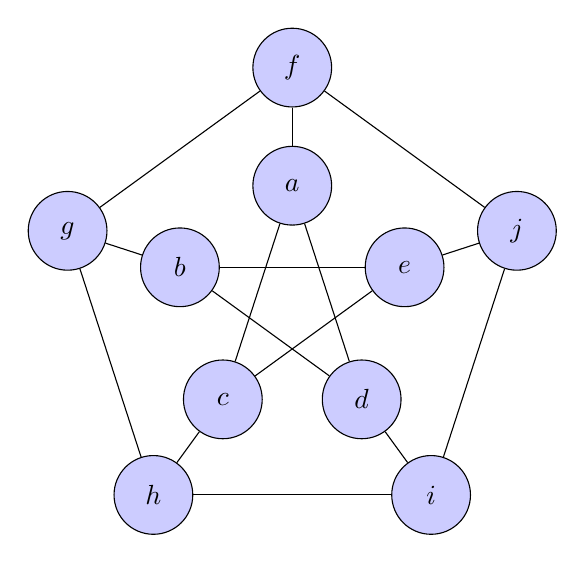
\begin{tikzpicture}[scale=1]
            \begin{scope}[rotate=90]
            \foreach \x/\y/\i in {0/1/a,72/2/b,144/3/c,216/4/d,288/5/e}{
                \node[main node] (\y) at (canvas polar cs:
                radius=1.5cm,angle=\x){$\i$};
            }
            \foreach \x/\y/\i in {0/6/f,72/7/g,144/8/h,216/9/i,288/10/j}{
                \node[main node] (\y) at (canvas polar cs: radius=3cm,angle=\x){$\i$};
            }
            \end{scope}
             
            \foreach \x/\y in {1/6,2/7,3/8,4/9,5/10}{
                \draw (\x) -- (\y);
            }
            \foreach \x/\y in {1/3,2/4,3/5,4/1,5/2}{
                \draw (\x) -- (\y);
            }
            \foreach \x/\y in {6/7,7/8,8/9,9/10,10/6}{
                \draw (\x) -- (\y);
            }
        \end{tikzpicture}
        \hspace{1cm}
        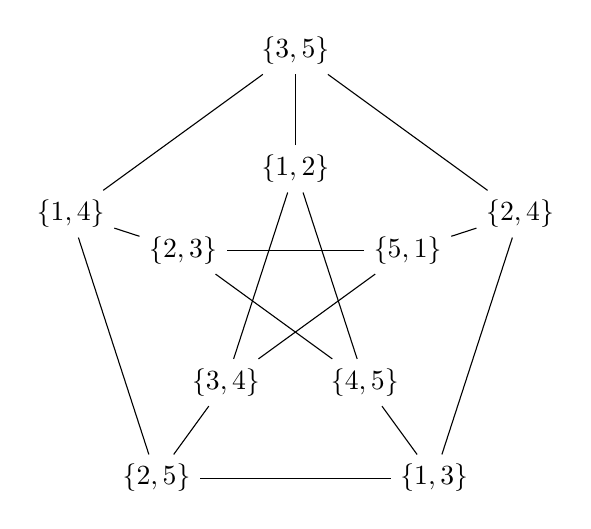
\begin{tikzpicture}[scale=1]
            \begin{scope}[rotate=90]
            \foreach \x/\y/\i/\j in {0/1/1/2,72/2/2/3,144/3/3/4,216/4/4/5,288/5/5/1}{
                \node (\y) at (canvas polar cs: radius=1.5cm,angle=\x){$\{\i, \j\}$};
            }
            \foreach \x/\y/\i/\j in {0/6/3/5,72/7/1/4,144/8/2/5,216/9/1/3,288/10/2/4}{
                \node (\y) at (canvas polar cs: radius=3cm,angle=\x){$\{\i, \j\}$};
            }
            \end{scope}
             
            \foreach \x/\y in {1/6,2/7,3/8,4/9,5/10}{
                \draw (\x) -- (\y);
            }
            \foreach \x/\y in {1/3,2/4,3/5,4/1,5/2}{
                \draw (\x) -- (\y);
            }
            \foreach \x/\y in {6/7,7/8,8/9,9/10,10/6}{
                \draw (\x) -- (\y);
            }
        \end{tikzpicture}
        \end{center}

        Let $\sigma$ be a permutation of $S$. This defined a corresponding
        permutation of the vertices, sending each vertex $\{x, y\} \to \{\sigma(x),
        \sigma(y)\}$. We claim that this is an automorphism of the graph. To see
        this, pick two vertices $\{x, y\}$, $\{p, q\}$. If they form an edge in $G$,
        that means that $x, y, p, q$ are all distinct elements, hence so are
        $\sigma(x), \sigma(y), \sigma(p), \sigma(q)$ meaning that $\{\sigma(x),
        \sigma(y)\}$, $\{\sigma(p), \sigma(q)\}$ is also an edge. Otherwise, one of
        these elements is repeated, hence applying $\sigma$ keeps them repeated so
        this maps non-edges to non-edges. Thus, we have found as many automorphisms
        of $G$ as there are permutations $\sigma$, i.e.\ $5! = 120$ of them.

        We now show that these are all the automorphisms of $G$. Note that the
        vertex $a \equiv \{1, 2\}$ can be mapped to any other vertex by choosing
        suitable $\sigma$, thus the orbit of $a$ comprises of all 10 vertices. The
        orbit stabilizer theorem thus guarantees that \[
            |\aut(G)| = |H|\cdot 10,
        \] where $H$ is the stabilizer of $a$. Now consider the action of $H$ on the
        graph, specifically on the vertex $c \equiv \{3, 4\}$. The permutation $(45)$
        sends $c \to f$, and $(35)$ sends $c \to d$. There are no other places to
        send $c$, since we must preserve the edge $\{a, c\}$. Thus, the orbit of $c$
        consists of the vertices $c, d, f$, hence \[
            |H| = |K|\cdot 3
        \] where $K$ is the stabilizer of $c$ under the action of $H$. Thus, the
        action of $K$ on the graph fixes both $a$ and $c$. Consider where $K$
        can send the vertex $d$. The permutation $(34)$ sends $d \to f$. There are no
        other places to send $d$, since we must preserve the edge $\{a, d\}$. Thus,
        the orbit of $d$ consists of the vertices $d, f$, hence \[
            |K| = |N|\cdot 2
        \] where $N$ is the stabilizer of $d$ under the action of $K$. Thus, the
        action of $N$ on the graph fixes $a, c, d$, which also means that $f$ must be
        fixed. Consider the action of $N$ on the graph, and examine the vertex $h$.
        The permutation $(12)$ sends $h \to e$, and there are no other places where
        $h$ can be sent. Thus, the orbit of $h$ consists of the vertices $h, e$,
        hence \[
            |N| = |O|\cdot 2,
        \] where $O$ is the stabilizer of $h$ under the action of $N$. Now, the
        action of $O$ on the graph fixes $a, c, d, h$. We claim that this also
        fixes all other elements, i.e.\ $O$ is the trivial group. Indeed, examining
        the neighbours of $c$ show that $a, h$ are fixed so $e$ must also be fixed.
        The vertex $i$ is the only common neighbour of $d$ and $h$, and hence must be
        fixed. Examining the neighbours of $h$ show that $c, i$ are fixed so $g$ must
        also be fixed. Similarly examining the neighbours of $i$ show that $d, h$ are
        fixed so $j$ must also be fixed. This means that the final vertex $f$ is also
        fixed. Thus, $|O| = 1$, hence \[
            |\aut(G)| = 10\cdot 3\cdot 2\cdot 2 = 120.
        \] 

    
    \problem Find the automorphism group of the following graphs.
    \begin{enumerate}
        \item \mbox{}
        \begin{center}
        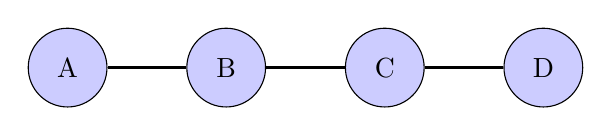
\begin{tikzpicture}[scale=1]
            \node[main node] (A) {A};
            \node[main node] (B) [right = 1cm of A] {B};
            \node[main node] (C) [right = 1cm of B] {C};
            \node[main node] (D) [right = 1cm of C] {D};

            \path[draw, thick]
            (A) edge (B)
            (B) edge (C)
            (C) edge (D);
        \end{tikzpicture}
        \end{center}

        \solution We first show that an automorphism must preserve the degree of a
        vertex. Indeed, given a vertex $x \in V(G)$ whose neighbours are $x_1, \dots,
        x_k$ ($k$ being the degree of $x$), if $g$ is an automorphism of the graph
        $G$ then $g(x_1), \dots, g(x_k)$ are all neighbours of $g(x)$; furthermore,
        the remaining vertices $y_1, \dots, y_l$ from $V(G)$ (vertices other than
        $x$, $x_1, \dots, x_k$) are also mapped such that $g(y_1), \dots, g(y_l)$ are
        not neighbours of $g(x)$ by construction of $g$.

        Secondly, an automorphism preserves edges. These two restrictions allow us to
        identify the automorphisms of the given graphs.

        Here, $B$ must be mapped to either $B$ or $C$. If $B \to B$, then $\{A, B\}
        \to \{X, B\}$ forcing $X = A$, hence $A \to A$. This also forces $C \to C$,
        and $D \to D$. Similarly if $B \to C$, then $\{A, B\} \to \{X, C\}$ forcing
        $X = D$, hence $A \to D$. This also forces $C \to B$, and $D \to A$.

        Thus, $\aut(G) \cong C_2$, the group with two elements.
        


        \item \mbox{}
        \begin{center}
        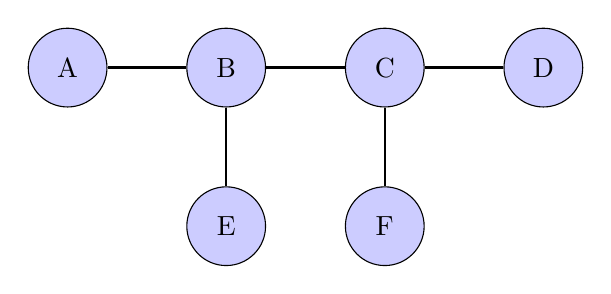
\begin{tikzpicture}[scale=1]
            \node[main node] (A) {A};
            \node[main node] (B) [right = 1cm of A] {B};
            \node[main node] (C) [right = 1cm of B] {C};
            \node[main node] (D) [right = 1cm of C] {D};
            \node[main node] (E) [below = 1cm of B] {E};
            \node[main node] (F) [below = 1cm of C] {F};

            \path[draw, thick]
            (A) edge (B)
            (B) edge (C)
            (C) edge (D)
            (B) edge (E)
            (C) edge (F);
        \end{tikzpicture}
        \end{center}

        \solution Note that if $B \to B$, we can have $(A, E) \to (A, E)$ or $(A, E)
        \to (E, A)$, either one independently of $(D, F) \to (D, F)$ or $(D, F) \to
        (F, D)$. (Here, $(X, Y) \to (P, Q)$ is shorthand for $X \to P$ and $Y \to
        Q$). By letting $e$ denote the identity permutation, $l$ denote the swap
        $(AB)$, $r$ denote the swap $(DF)$, and $c$ denote the permutation
        $(BC)(AD)(EF)$, we can see that $\aut(G)$ consists of the following elements:
        \[
            e, r, l, rl, c, rc, lc, rlc.
        \] In other words, \[
            \aut(G) = \{e, r\} \times \{e, l\} \times \{e, c\} \cong C_2\times
            C_2\times C_2.
        \] 
        

        \item \mbox{}
        \begin{center}
        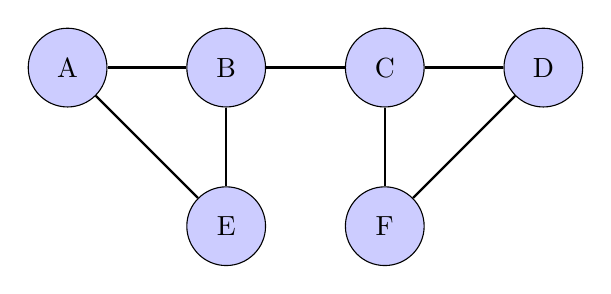
\begin{tikzpicture}[scale=1]
            \node[main node] (A) {A};
            \node[main node] (B) [right = 1cm of A] {B};
            \node[main node] (C) [right = 1cm of B] {C};
            \node[main node] (D) [right = 1cm of C] {D};
            \node[main node] (E) [below = 1cm of B] {E};
            \node[main node] (F) [below = 1cm of C] {F};

            \path[draw, thick]
            (A) edge (B)
            (B) edge (C)
            (C) edge (D)
            (B) edge (E)
            (E) edge (A)
            (C) edge (F)
            (F) edge (D);
        \end{tikzpicture}
        \end{center}
        
        \solution The arguments in the previous solution remain unchanged, with \[
                \aut(G) = \{e, r\} \times \{e, l\} \times \{e, c\} \cong C_2\times
                C_2\times C_2.
        \] 



        \item \mbox{}
        \begin{center}
        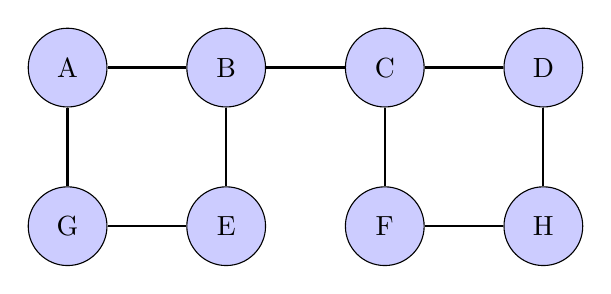
\begin{tikzpicture}[scale=1]
            \node[main node] (A) {A};
            \node[main node] (B) [right = 1cm of A] {B};
            \node[main node] (C) [right = 1cm of B] {C};
            \node[main node] (D) [right = 1cm of C] {D};
            \node[main node] (E) [below = 1cm of B] {E};
            \node[main node] (F) [below = 1cm of C] {F};
            \node[main node] (G) [below = 1cm of A] {G};
            \node[main node] (H) [below = 1cm of D] {H};

            \path[draw, thick]
            (A) edge (B)
            (B) edge (C)
            (C) edge (D)
            (B) edge (E)
            (E) edge (G)
            (G) edge (A)
            (C) edge (F)
            (F) edge (H)
            (H) edge (D);
        \end{tikzpicture}
        \end{center}

        \solution If $B \to B$, then $A$ can be mapped to either $A, E$ and $E$ gets
        the remaining spot. Similarly, $C$ can be mapped to either $C, H$ and $H$
        gets the remaining spot. The places of $G$ and $H$ are fixed. There is an
        analogous case when $B \leftrightarrow C$. Thus, define the permutations $l =
        (AE)$, $r = (DF)$, $c = (BC)(AD)(EF)(GH)$. Then, \[
            \aut(G) = \{e, r\} \times \{e, l\} \times \{e, c\} \cong C_2\times
            C_2\times C_2.
        \] 


        \item \mbox{}
        \begin{center}
        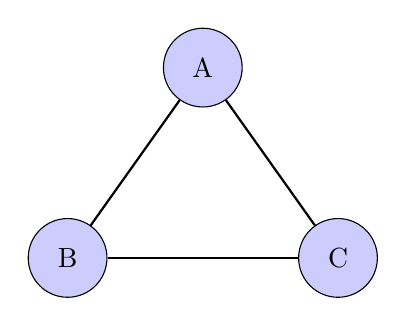
\begin{tikzpicture}[scale=1]
            \node[main node] (A) {A};
            \node[main node] (B) [below left = 1.7cm and 1cm of A] {B};
            \node[main node] (C) [below right = 1.7cm and 1cm of A] {C};
            
            \path[draw, thick]
            (A) edge (B)
            (B) edge (C)
            (C) edge (A);
        \end{tikzpicture}
        \end{center}

        \solution It is clear that any permutation of $A, B, C$ gives a graph
        automorphism, since this is the connected graph $K_3$. Thus, \[
            \aut(G) \cong S_3.
        \] 


        \item \mbox{}
        \begin{center}
        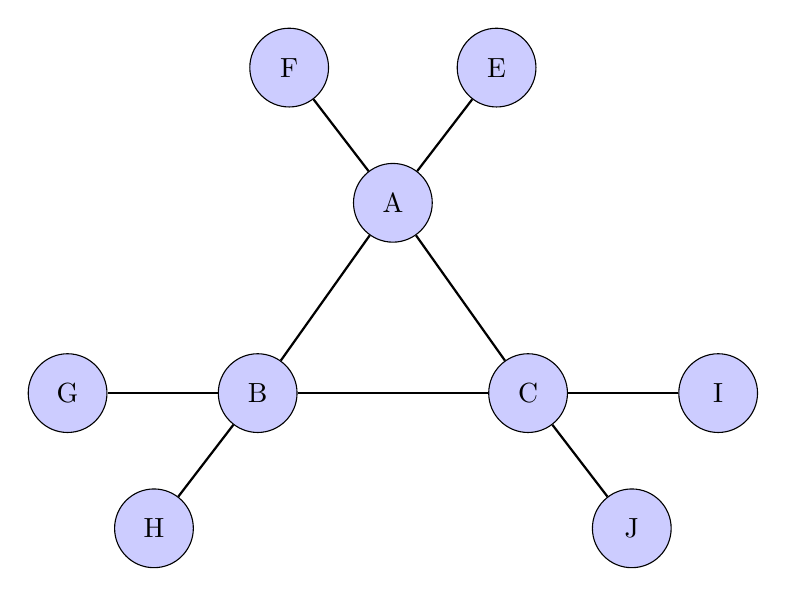
\begin{tikzpicture}[scale=1]
            \node[main node] (A) {A};
            \node[main node] (B) [below left = 1.7cm and 1cm of A] {B};
            \node[main node] (C) [below right = 1.7cm and 1cm of A] {C};
            \node[main node] (E) [above right = 1cm and 0.6cm of A] {E};
            \node[main node] (F) [above left = 1cm and 0.6cm of A] {F};
            \node[main node] (G) [left = 1.4cm of B] {G};
            \node[main node] (H) [below left = 1cm and 0.6cm of B] {H};
            \node[main node] (I) [right = 1.4cm of C] {I};
            \node[main node] (J) [below right = 1cm and 0.6cm of C] {J};
            
            \path[draw, thick]
            (A) edge (B)
            (A) edge (E)
            (A) edge (F)
            (B) edge (C)
            (B) edge (G)
            (B) edge (H)
            (C) edge (A)
            (C) edge (I)
            (C) edge (J);
        \end{tikzpicture}
        \end{center}

        \solution Like before, $A, B, C$ can be permuted in any way. After this, $E,
        F$ can occupy the two positions next to where $A$ lands in 2 ways, and the
        same goes for $G, H$ next to $B$, $I, J$ next to $C$. Thus, \[
            \aut(G) \cong S_3\times C_2 \times C_2 \times C_2.
        \] 
        
        \item \mbox{}
        \begin{center}
        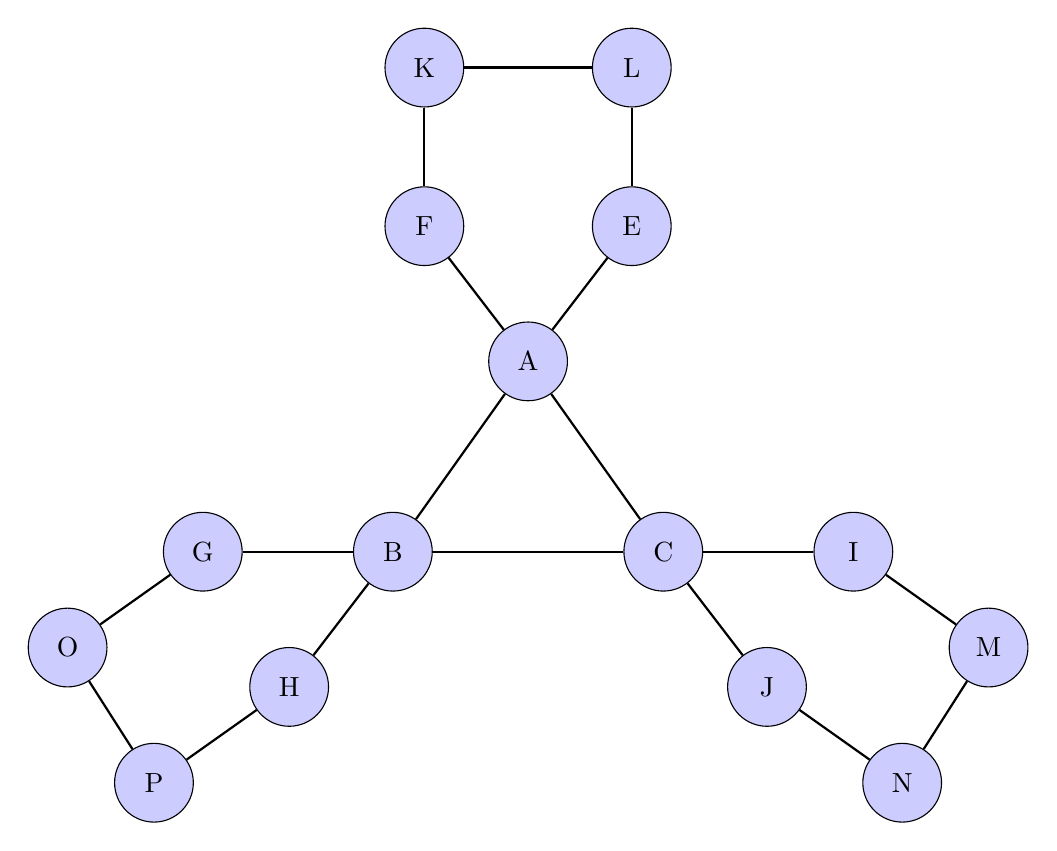
\begin{tikzpicture}[scale=1]
            \node[main node] (A) {A};
            \node[main node] (B) [below left = 1.7cm and 1cm of A] {B};
            \node[main node] (C) [below right = 1.7cm and 1cm of A] {C};
            \node[main node] (E) [above right = 1cm and 0.6cm of A] {E};
            \node[main node] (F) [above left = 1cm and 0.6cm of A] {F};
            \node[main node] (G) [left = 1.4cm of B] {G};
            \node[main node] (H) [below left = 1cm and 0.6cm of B] {H};
            \node[main node] (I) [right = 1.4cm of C] {I};
            \node[main node] (J) [below right = 1cm and 0.6cm of C] {J};
            \node[main node] (K) [above = 1cm of F] {K};
            \node[main node] (L) [above = 1cm of E] {L};
            \node[main node] (O) [below left = 0.5cm and 1cm of G] {O};
            \node[main node] (P) [below left = 0.5cm and 1cm of H] {P};
            \node[main node] (M) [below right = 0.5cm and 1cm of I] {M};
            \node[main node] (N) [below right = 0.5cm and 1cm of J] {N};
            
            \path[draw, thick]
            (A) edge (B)
            (A) edge (E)
            (A) edge (F)
            (F) edge (K)
            (K) edge (L)
            (L) edge (E)
            (B) edge (C)
            (B) edge (G)
            (B) edge (H)
            (H) edge (P)
            (P) edge (O)
            (O) edge (G)
            (C) edge (A)
            (C) edge (I)
            (C) edge (J)
            (J) edge (N)
            (N) edge (M)
            (M) edge (I);
        \end{tikzpicture}
        \end{center}

        \solution We repeat exactly the same arguments as before: $A, B, C$ permute
        freely, the elements $F, E$ attach to $A$ in two ways, and the remaining lobe
        $K, L$ is forced by the positioning of $F, E$. Thus we have \[
            \aut(G) \cong S_3\times C_2 \times C_2 \times C_2.
        \] 

    \end{enumerate}


    \problem Find the orbits of all the vertices of the following graphs.

    \begin{enumerate}
        \item \mbox{}
        \begin{center}
        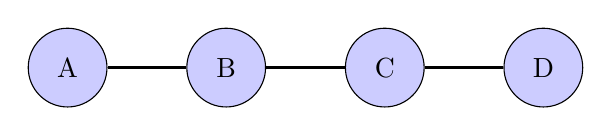
\begin{tikzpicture}[scale=1]
            \node[main node] (A) {A};
            \node[main node] (B) [right = 1cm of A] {B};
            \node[main node] (C) [right = 1cm of B] {C};
            \node[main node] (D) [right = 1cm of C] {D};

            \path[draw, thick]
            (A) edge (B)
            (B) edge (C)
            (C) edge (D);
        \end{tikzpicture}
        \end{center}

        \solution Recall that we have computed the automorphism group of this graph.
        The orbits are \[
            \{B, C\}, \qquad \{A, D\}.
        \] In other words, the orbit of $B$ and the orbit of $C$ is $\{B, C\}$; the
        orbit of $A$ and the orbit of $D$ is $\{A, D\}$.


        \item \mbox{}
        \begin{center}
        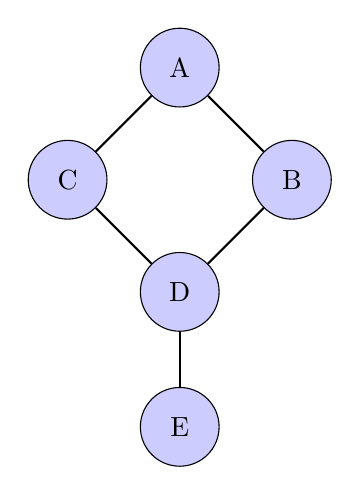
\begin{tikzpicture}[scale=1]
            \node[main node] (A) {A};
            \node[main node] (B) [below right = 1cm of A] {B};
            \node[main node] (C) [below left = 1cm of A] {C};
            \node[main node] (D) [below left = 1cm of B] {D};
            \node[main node] (E) [below = 0.7cm of D] {E};

            \path[draw, thick]
            (A) edge (B)
            (A) edge (C)
            (B) edge (D)
            (C) edge (D)
            (D) edge (E);
        \end{tikzpicture}
        \end{center}

        \solution Note that $D$ can only be mapped to $D$, $A$ can only be mapped
        to $A$, and $E$ only to $E$. The permutation $(BC)$ does give an
        automorphism. Thus, the orbits are \[
            \{A\}, \qquad \{B, C\}, \qquad \{E\}, \qquad \{E\}.
        \] 

        \item \mbox{}
        \begin{center}
        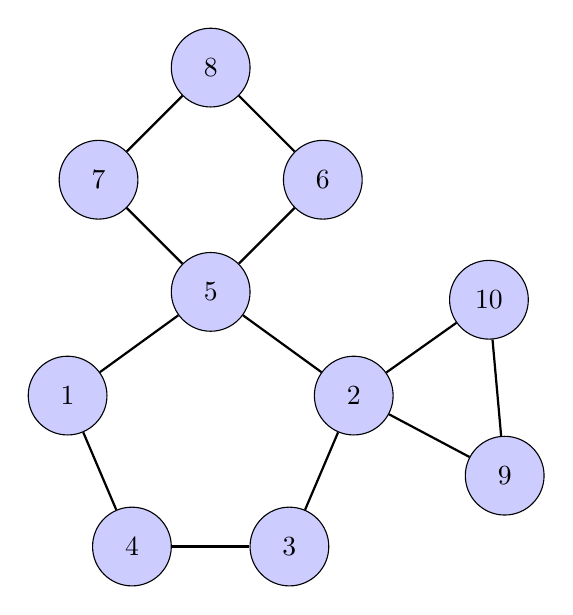
\begin{tikzpicture}[scale=1]
            \node[main node] (8) {8};
            \node[main node] (6) [below right = 1cm of 8] {6};
            \node[main node] (7) [below left = 1cm of 8] {7};
            \node[main node] (5) [below left = 1cm of 6] {5};
            \node[main node] (1) [below left = 0.6cm and 1.1cm of 5] {1};
            \node[main node] (2) [below right = 0.6cm and 1.1cm of 5] {2};
            \node[main node] (4) [below right = 1.2cm and 0.1cm of 1] {4};
            \node[main node] (3) [below left = 1.2cm and 0.1cm of 2] {3};
            \node[main node] (10) [above right = 0.5cm and 1cm of 2] {10};
            \node[main node] (9) [below right = 0.3cm and 1.2cm of 2] {9};

            \path[draw, thick]
            (8) edge (6)
            (6) edge (5)
            (5) edge (7)
            (7) edge (8)
            (5) edge (1)
            (1) edge (4)
            (4) edge (3)
            (3) edge (2)
            (2) edge (5)
            (2) edge (9)
            (9) edge (10)
            (10) edge (2);
        \end{tikzpicture}
        \end{center}

        \solution Note that if 5 is mapped to 2, then 6,7 must be mapped to 9, 10
        leaving no room for mapping 8. Thus, 5 must remain fixed, 2 must remain
        fixed. 6 and 7 must be mapped amongst themselves; if say 6 is mapped to 1,
        then 8 must be mapped to 4, 7 to 3 which breaks the edge $7 \sim 5$. Thus, 8
        must remain fixed. This in turn fixes 1, 3, 4. Finally, 9 and 10 can be
        mapped amongst themselves. The orbits are \[
            \{1\}, \{2\}, \{3\}, \{4\}, \{5\}, \{6, 7\}, \{8\}, \{9, 10\}.
        \] 


    \end{enumerate}




    \problem Prove that the $n$-cube is vertex transitive for any $n \in \N$.

    \solution Label the each vertex of the $n$-cube with binary strings of length
    $n$, i.e.\ let each vertex be denoted by $x \equiv x_1x_2 \dots x_n$ where each
    $x_i \in \{0, 1\}$. Two vertices are adjacent if and only if they differ in
    exactly one place, i.e.\ one bit.

    Denote the bit complements $a' = 1 - a$ ($0' = 1$ and $1' = 0$). Define the bit
    flip operations $f_i\colon V \to V$, where $x \mapsto x_1x_2 \dots x_{i -
    1}x_i'x_{i + 1} \dots x_n$. In other words, $f_i$ flips the $i$th bit of each
    vertex. It is clear that this is a bijection: no two vertices can be mapped to
    the same vertex, and every vertex has a pre-image. Indeed, $f_i^2(x) = x$ because
    $a'' = a$ for any bit $a$; this proves both injectivity\footnote{If $f_i(x) =
    f_i(y)$, then $f_i^2(x) = f_i^2(y)$ gives $x = y$.} and surjectivity\footnote{The
    pre-image of $x$ is $f_i(x)$.}. Furthermore, we claim that each $f_i$ is an
    automorphism of the $n$-cube. To see this, pick two vertices $x$ and $y$, and
    suppose that they differ in $k$ bits. Specifically, if $x_i = y_i$, then $x_i' =
    y_i'$; if $x_i \neq y_i$, then $x_i' \neq y_i'$. This shows that $f_i(x)$ and
    $f_i(y)$ still differ in $k$ bits. Thus, $f_i$ preserves the edges of the
    $n$-cube.

    Now, pick an arbitrary vertex $x$. Suppose that the binary string of $x$ has 1's
    in precisely the indices $i_1, i_2, \dots, i_k$. Then, it is clear that
    $f_{i_1}\circ f_{i_2}\circ \dots \circ f_{i_k}(x) = 0$ (the vertex whose binary
    string only consists of 0's). Note that this composition of automorphisms is
    itself an automorphism. Thus, every vertex $x$ contains the common vertex $0$ in
    its orbit, proving that the $n$-cube is vertex transitive.


    \problem If $G$ is a vertex transitive simple connected graph of order $\geq 3$,
    then prove that $G$ does not contain a cut-vertex.

    \solution Note that such a graph is regular (an automorphism preserves the
    degrees of each vertex) with minimum degree $2$. The latter follows because if
    every vertex had degree $1$, then given an edge $\{x, y\}$, there can be no path
    from $x$ to a third vertex $z$: neither $x$ nor $y$ can contribute another edge.     

    First, we claim that an automorphism of $G$ cannot map a non cut-vertex to a
    cut-vertex. Let $x$ not be a cut-vertex, and suppose that $g \in \aut(G)$ is such
    that $g(x)$ is a cut vertex. This means that there exist vertices $y', z'$ such
    that every path between them passes through $g(x)$. Set $y = g^{-1}(y')$, $z =
    g^{-1}(z')$; since $x$ is not a cut vertex, there exists  a path $y, v_1, \dots,
    v_k, z$ not passing through $x$. The image, $y', g(v_1), \dots, g(v_k), z'$ is
    still a path, and none of the $g(v_i) = g(x)$ since that would imply $v_i = x$.
    This contradicts the fact that $g(x)$ is a cut vertex.

    Next, we claim that every connected graph has a non cut-vertex. The lemmas proved
    in Assignment 3 show that every connected graph $G$ has a spanning tree, and
    every tree contains a leaf -- pick such a spanning tree $T$ and a leaf $x$. Now
    pick two vertices $y, z$ from $G$; since $T$ is a spanning tree, there exists a
    path between $y$ and $z$ within the tree $T$ i.e.\ only using edges from $T$.
    Such a path cannot include the vertex $x$: note that $x$ is not an endpoint of
    the path, but $x$ has degree 1 so it cannot be an intermediate vertex in the path
    either. Thus, the removal of $x$ still keeps $T$, hence $G$ connected, which
    means that $x$ is not a cut-vertex.

    The above immediately show that a vertex transitive simple connected graph cannot
    contain a cut-vertex: simply pick a non cut-vertex and note that it can be mapped
    to any other vertex via an automorphism. Thus, none of these vertices can be a
    cut-vertex either.


    \problem Prove that the group action of the automorphism group of a vertex
    transitive graph on the vertex set of the graph can have only one orbit.

    \solution Let $G$ be a vertex transitive graph and let $x \in V(G)$. Then, for
    any $y \in V(G)$, there exists an automorphism $g \in \aut(G)$ such that $gx =
    y$. In other words, $y$ is in the orbit of $x$ for all $y \in V(G)$, so the orbit
    of $x$ is all of $V(G)$. This is true for any $x \in V(G)$, hence there is only
    one orbit.


    \problem Prove that \[
        \chi(G) \geq \frac{|V(G)|}{\alpha(G)}.
    \] 
    
    \solution Let the vertices of $G$ be coloured (in the proper manner) in $k =
    \chi(G)$ colours, and let $V_1, \dots, V_k$ be sets of vertices where $V_i$
    contains vertices of the $i$th colour. This is a partition of the vertices of
    $G$. Furthermore, each $V_i$ is an independent set by construction: no two
    vertices of the same colour are adjacent. Thus, $\alpha(G) \geq |V_i|$ for each
    $i$, giving \[
        k\cdot \alpha(G) \geq \sum_{i = 1}^k |V_i| = |V(G)|
    \] as desired.



    \problem Construct a graph $G$ that is neither a clique nor an odd cycle but has
    a vertex ordering relative to which the greedy colouring uses $\Delta(G) + 1$
    colours.

    \solution Let $G$ be the following graph, with vertices labelled 1,\dots, 6 and
    colours Red, Green, Blue in order.
    \begin{center}
    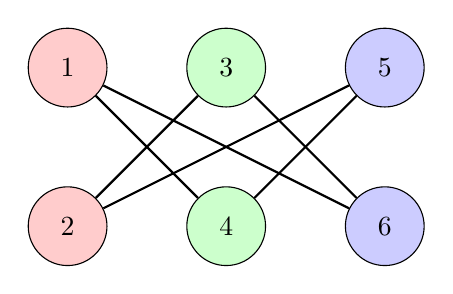
\begin{tikzpicture}[scale=1]
        \node[red node] (1) {1};
        \node[red node] (2) [below = 1cm of 1] {2};
        \node[green node] (3) [right = 1cm of 1] {3};
        \node[green node] (4) [below = 1cm of 3] {4};
        \node[main node] (5) [right = 1cm of 3] {5};
        \node[main node] (6) [below = 1cm of 5] {6};

        \path[draw, thick]
        (1) edge (4)
        (1) edge (6)
        (3) edge (2)
        (3) edge (6)
        (5) edge (2)
        (5) edge (4);
    \end{tikzpicture}
    \end{center}
    It is easily checked that this is indeed the colouring produced by the greedy
    algorithm; after colouring 1, 2 in red, 3, 4 must be given a new colour and 5, 6
    yet another new colour. Thus, we have used $3 = \Delta(G) + 1$ colours. However,
    it is clear that $\chi(G) = 2$ since it is bipartite.
    
    \problem Prove that a graph $G$ is $2^k$-colourable if and only if $G$ is the
    union of $k$ bipartite graphs.

    \solution First suppose that $G$ is the union of $k$ bipartite graphs, $G_1,
    \dots, G_k$. Let the two parts of each $G_i$ be $A_i$ and $B_i$. Without loss of
    generality, let $V(G) = V(G_i)$ --- do this by adding any remaining vertices not
    in $G_i$ to the part $A_i$, and note that this keeps each $G_i$ bipartite (we
    aren't adding any new edges). Now, given a vertex $x$ in $G$ and an index $i$,
    $x$ is present in exactly one of $A_i$ or $B_i$.  Define $x_i = 1$ if $x \in
    A_i$, and $x_i = 0$ if $x \in B_i$. In this manner, colour each vertex $x \in G$
    with the binary string $x_1x_2 \dots x_k$. There are at most $2^k$ possible
    colours. We now show that this is indeed a proper colouring of $G$. To do this,
    suppose that two vertices $x$ and $y$ have the same colour, i.e.\ their binary
    strings match. For each index $i$, we have $x_i = y_i$; if this is 1, then $x, y
    \in A_i$ and if this is 0, then $x, y \in B_i$. In either case, $x, y$ belong to
    the same part in $G_i$, hence $G_i$ does not contribute the edge $\{x, y\}$.
    However, every edge in $G$ must come from some $G_i$, since it is the union of
    all $G_i$; this proves that $G$ does not contain the edge $\{x, y\}$, hence our
    colouring is proper.

    Next, suppose that $G$ is $2^k$-colourable; like before, label these colours with
    binary strings of length $k$ and colour each vertex with them. For each index $1
    \leq i \leq k$, create the sets $A_i$ and $B_i$. Now given a vertex $x$ in $G$,
    look at the $i$th place in the binary string, i.e.\ the bit $x_i$, and define $x
    \in A_i$, $x \notin B_i$ if $x_i = 1$, otherwise $x \notin A_i$, $x \in B_i$ if
    $x_i = 0$. Finally, construct each $G_i$ by starting with $G$, then removing all
    edges within $A_i$ (that is, removing all edges with both endpoints in $A_i$) and
    removing all edges within $B_i$. Note that each $G_i$ is clearly bipartite by
    construction. We now claim that their union gives all of $G$, i.e.\ every edge in
    $G$ can be found in some $G_i$. Indeed, pick an edge $\{x, y\}$ from $G$; note
    that by our colouring scheme, $x$ and $y$ must have different colours, hence
    their binary strings differ in some index $i$, with $x_i \neq y_i$. Thus, $x_i
    \in A_i$ and $y_i \in B_i$ (without loss of generality), so $G_i$ contains the
    edge $\{x, y\}$ (we have not removed this edge when constructing $G_i$).



    \problem Prove that every graph $G$ has a vertex ordering relative to which the
    greedy colouring uses $\chi(G)$ colours.

    \solution Let $G$ be coloured using $k = \chi(G)$ colours, and let $V_1, \dots,
    V_k$ be the sets of vertices of $G$ such that $V_i$ contains vertices of the
    $i$th colour. Then, each $V_i$ is an independent set. Now, label the vertices of
    each $V_i$ in any order, as $V_i = \{v_{i1}, v_{i2}, \dots, v_{it}\}$. Finally,
    label the vertices of $G$ in order $[V_1, V_2, \dots, V_k]$, i.e.\ $v_{11},
    v_{12}, \dots, v_{1t_1}, v_{21}, v_{22}, \dots, v_{kt_k}$. Here, the vertices
    appear sorted in ascending order of their colour. 

    Now, apply the greedy algorithm. For the first $t_1$ vertices taken from $V_1$,
    all can be assigned the lowest in index colour 1, since there are no conflicts
    ($V_1$ is independent). Next introduce the vertices from $V_2$; here, each vertex
    can be coloured with either 1, 2. There is no need to introduce the colour 3
    since no vertex from $V_2$ is connected to another from $V_2$, which means that
    they are only connected to vertices from $V_1$ coloured in 1. Similarly, at the
    stage when vertices of $V_{j + 1}$ are introduced, the previous vertices all
    being given colours $1,\dots,j$, note that each new vertex can be given a colour
    from $1,\dots,j,j+1$ since they are only connected to vertices from vertices from
    $V_1,\dots,V_j$ coloured in $1,\dots,j$. This shows that the greedy algorithm
    will terminate by using only $k = \chi(G)$ colours.


    \problem Prove that $\chi(G) = \omega(G)$ when $\overline{G}$ is bipartite, where
    $\omega(G)$ is the maximum size of a set of pairwise adjacent vertices (called a
    clique) in $G$.

    \solution Recall that if any subgraph od $G$ has chromatic number $k$, then
    $\chi(G) \geq k$ (otherwise would imply the $< k$ colorability of the subgraph).
    Let $X$ be a largest clique in $G$ of $\omega(G)$ vertices; we have $\chi(G) \geq
    \omega(G)$.
    

    \problem Prove that every $k$-chromatic graph has at least $\binom{k}{2}$ edges.
    Use this to prove that if $G$ is the union of $m$ complete graphs of order $m$,
    then $\chi(G) \leq 1 + m\sqrt{m - 1}$.

    \solution First, let $G$ be $k$-chromatic, and let $V_1, \dots, V_k$ be the
    vertex sets where $V_i$ contains vertices of the $i$th colour. Examine any pair
    $V_i, V_j$, with $i \neq j$. Suppose that there is no edge between them (there is
    no edge with one endpoint in $V_i$, the other in $V_j$). Then, recolouring $V_j$
    to be the same colour as $V_i$ gives us a proper $k - 1$ colouring of $G$,
    contradicting the minimality of $k$. Thus, there must be at least one edge
    associated with each pair $i, j$, of which there are $\binom{k}{2}$.

    Now, let $G$ be the union of $m$ complete graphs of order $m$. Then, $G$ has at
    most $m \cdot \binom{m}{2}$ edges. Set $\chi(G) = k$, hence \[
        m\cdot \binom{m}{2} \geq |E(G)| \geq \binom{k}{2}, \qquad 
        m^2(m - 1) \geq k(k - 1) \geq (k - 1)^2.
    \] Taking a square root, $k - 1 \leq m\sqrt{m - 1}$ or $k \leq 1 + m\sqrt{m - 1}$
    as desired. \\


    \begin{lemma}
        The chromatic polynomial of a graph with two components is the product of the
        chromatic polynomials of those components.
    \end{lemma}
    \begin{proof}
        Let $G_1$, $G_2$ be the two components of $G$. Then, there are no edges
        between them. Given some $k$, there are $P_{G_1}(k)$ ways of colouring $G_1$,
        and for each of these there are $P_{G_2}(k)$ ways of colouring $G_2$. This
        gives a total of $P_{G_1}(k)P_{G_2}(k)$ colourings of $G$. Furthermore, every
        colouring of $G$ can be expressed in this way, i.e.\ every colouring of $G$
        gives a colouring of $G_1$ and a colouring of $G_2$, hence we have accounted
        for all possible $k$-colourings of $G$.
    \end{proof}


    \problem Prove that if $T$ is a tree with $n$ vertices, then $P_T(k) = k(k -
    1)^{n - 1}$.

    \solution We use induction on $n$. This is trivial for $n = 2$, since the tree on
    $2$ vertices clearly shows $P_T(k) = k(k - 1)$. Now, pick a tree $T$ with $n > 2$
    vertices, and suppose that this statement holds for all trees with less than $n$
    vertices. Let $x$ be a leaf of $T$, and let $e = \{x, y\}$ be the only edge of
    $x$. Then, $T' = T / e$ is a tree on $n - 1$ vertices. Furthermore, $T - e$ gives
    the same tree $T'$ along with an extra isolated vertex $x$. Using the relation
    $P_{G} = P_{G - e} - P_{G/e}$ together with Lemma 1 (the chromatic polynomial of
    a single isolated vertex is just $k$), we can write \[
        P_T(k) = k \cdot P_{T'}(k) - P_{T'}(k) = (k - 1)P_{T'}(k) = (k - 1)\cdot k(k
        - 1)^{n - 2} = k(k - 1)^{n - 1}.
    \] 


    \problem Show that the chromatic polynomial $P_G(k)$ has degree $|V(G)|$, with
    integer coefficients alternating in sign and beginning $1, -e(G), \dots, $. Here,
    $e(G)$ is the number of edges in $G$.

    \solution This is easily verified for all graphs $G$ with at most $2$ vertices.
    We proceed by induction on $n$; suppose that this holds for all graphs will fewer
    than $n > 2$ vertices. Pick a graph $G$ on $n$ vertices. If $e(G) = 0$, i.e.\ $G$
    only contains isolated vertices, it is clear that $P_G(k) = k^n$ which is of the
    given form. Otherwise, we perform induction on $e(G)$; suppose that this
    statement holds for all $G$ with $n$ vertices, and fewer than $e(G)$ edges. Pick
    an edge $e$ from $G$, and note that $G - e$ has $n$ vertices, $e(G) - 1$ edges
    while $G/e$ has $n - 1$ vertices. Thus, write their chromatic polynomials as 
    \begin{align*}
        P_{G - e}(k) &= k^n - (e(G) - 1)k^{n - 1} + a_{n - 2}k^{n - 2} + a_{n - 3}k^{n
        - 3} - \dots + (-1)^na_0, \\
        P_{G/e}(k) &= k^{n - 1} - b_{n - 2}k^{n - 2} + b_{n - 3}k^{n - 3} + \dots +
        (-1)^{n - 1}b_0.
    \end{align*}
    Here, all $a_i, b_i \geq 0$. Using $P_{G} = P_{G - e} - P_{G/e}$ gives us \[
        P_G(k) = k^n - e(G)k^{n - 1} + (a_{n - 2} + b_{n - 2})k^{n - 2} - (a_{n - 3}
        + b_{n - 3})k^{n - 3} + \dots + (-1)^n(a_0 + b_0),
    \] which is of the desired form.



    \problem Prove that $k^4 - 4k^3 + 3k^2$ is not a chromatic polynomial.

    \solution Denote this expression as $p(k)$. Note that \[
        p(k) = k^2(k^2- 4k + 3) = k^2(k - 1)(k - 3).
    \] If $p$ was the chromatic polynomial of some graph $G$, this would imply that
    $G$ has $p(3) = 0$ number of 3-colourings, but $p(2) = -4$ number of
    2-colourings, which is absurd.


    \problem Prove that \[
        P_{C_n}(k) = (k - 1)^n + (-1)^n(k - 1).
    \] 

    \solution We show this by induction. This is clearly true for $n = 3$, since
    there are $k\cdot(k - 1)\cdot(k - 2)$ ways of colouring $C_3 = K_3$ with $k$
    colours, and this is just $k^3 - 3k^2 + 2k = (k - 1)^3 - (k - 1)$.

    Now, suppose that this holds for cycles of length less than $n > 3$. Pick an edge
    $e$ from $C_n$, and note that $C_n - e = P_n$, $C_n / e = C_{n - 1}$. Thus, our
    reduction formula gives \[
        P_{C_n}(k) = P_{P_n}(k) - P_{C_{n - 1}}(k) = k(k - 1)^{n - 1} - \left[(k -
        1)^{n - 1} + (-1)^{n - 1}(k - 1)\right].
    \] Simplifying, this gives \[
        P_{C_n}(k) = (k - 1)^{n - 1}(k - 1) - (-1)^{n - 1}(k - 1) = (k - 1)^n +
        (-1)^n(k - 1).
    \] 

    \begin{lemma}
        The chromatic polynomial of any graph has integer coefficients.
    \end{lemma}
    \begin{proof}
        Use the induction method of Exercise 16; if all the coefficients of $P_{G -
        e}$ and $P_{G / e}$ are integers, then so are the coefficients of $P_G$.
    \end{proof}

    \begin{lemma}
        The chromatic polynomial of any graph can only have integer roots.
    \end{lemma}
    \begin{proof}
        This follows directly from the rational root theorem. Suppose that \[
            P_G(k) = k^t\left[k^{n - t} - mk^{n - t - 1} + \dots + a_1k + a_0\right],
        \] where $a_0 \neq 0$ (if $P_G$ has no such coefficient, then $P_G(k) = k^n$
        and we are done). Then, the roots of the bracketed polynomial must be
        rational numbers $p / q$, $\gcd(p, q) = 1$ such that $p | a_0$ and $q | 1$,
        i.e.\ the roots must be integers. This is also easily seen from the fact that
        if \[
             k^{n - t} - mk^{n - t - 1} + \dots + a_1k + a_0 = 0,
        \] all the powers of $k$ are divisible by $k$, hence $a_0$ must also be
        divisible by $k$.
    \end{proof}


    \problem Prove that the chromatic polynomial of an $n$-vertex graph has no real
    root larger than $n - 1$.

    \solution Note that $\chi(G) \leq n$ for any graph, hence its chromatic
    polynomial $P_G(k)$ is a strictly positive integer for all integers $k \geq n$
    (any $\chi(G)$ colouring gives a valid $k \geq n$ colouring). Thus, $P_G$ has no
    integer roots $k > n - 1$; but $P_G$ can only have integer roots by the above
    lemma, so $P_G$ has no real roots $x > n - 1$.


    \begin{lemma}
        The chromatic polynomial of any graph has no negative roots.
    \end{lemma}
    \begin{proof}
        Since the coefficients of $P_G$ have alternating signs, $P_G(k)$ for negative
        $k$ is strictly positive when the degree $n$ is even, and strictly negative
        when the degree $n$ is odd. Hence, there can be no negative roots.
    \end{proof}

    \begin{lemma}
        The roots of a chromatic polynomial must among the integers $0, 1, \dots,
        \chi(G) - 1$.
    \end{lemma}


        
    \problem Prove that the last non-zero term in the chromatic polynomial of $G$ is
    the term whose exponent is the number of components of $G$.

    \solution We will show that when $G$ is connected, the highest power of $k$
    dividing $P_G(k)$ is exactly $k$. This in turn will show that when $G$ has $r$
    components, the highest power of $k$ dividing $P_G(k)$ will be $k^r$ (Lemma 1
    shows that the chromatic polynomials of the components multiply).

    Let $G$ be a connected graph on $n$ vertices. Then it is clear that $P_G(0) = 0$
    since there is no way of colouring $G$ with zero colours, thus $k | P_G(k)$.
    Another way to see this is to note that for any $k \geq \chi(G)$ and given some
    proper $k$-colouring of $G$, cyclically permuting the $k$ colours yields $k$
    distinct proper colourings.  Furthermore, none of these can be obtained by
    cyclically permuting the colours of some other $k$-colouring not present here.
    Thus, the $P_G(k)$ many $k$-colourings can be partitioned into groups of $k$,
    hence $k | P_G(k)$.

    Note that the highest power of $k$ dividing the chromatic polynomial of any
    connected graphs on $2$ vertices is just $k$, as desired. Suppose that this
    result holds for all connected graphs on fewer than $n > 2$ vertices, and let $G$
    be connected with $n$ vertices. If $G$ has $n - 1$ edges, it is a tree so we know
    that $P_G(k) = k(k - 1)^{n - 1}$. Further suppose that the result holds for all
    $G$ on fewer than $n$ vertices, fewer than $e(G) > n - 1$ edges. Since $e(G) > n
    - 1$, it contains a cycle. Then, we can find an edge $e$ whose removal keeps $G$
    connected (there are edges in $G$ apart from those in its spanning tree, choose
    one of these). Now, $G - e$ is connected with fewer than $e(G)$ edges, and $G /
    e$ is connected with fewer than $n$ vertices. Thus, write
    \begin{align*}
        P_{G - e}(k) &= k^n - (e(G) - 1)k^{n - 1} + a_{n - 2}k^{n - 2} + a_{n - 3}k^{n
        - 3} - \dots - (-1)^na_1k, \\
        P_{G/e}(k) &= k^{n - 1} - b_{n - 2}k^{n - 2} + b_{n - 3}k^{n - 3} + \dots -
        (-1)^{n - 1}b_1k.
    \end{align*}
    Here, all $a_i, b_i \geq 0$ and $a_1, b_1 \neq 0$ since $k^2$ does not divide
    either of these polynomials by the induction hypothesis. Subtracting, \[
        P_G(k) = k^n - e(G)k^{n - 1} + (a_{n - 2} + b_{n - 2})k^{n - 2} - (a_{n - 3}
        + b_{n - 3})k^{n - 3} + \dots - (-1)^n(a_1 + b_1)k.
    \] Again, $a_1 + b_1 \neq 0$ hence $k^2$ does not divide $P_G(k)$. This proves the
    result by induction.
 
\end{document}
